\section{Software Design Patterns}
\label{sec:design_patterns}

To address recurring design challenges and enhance the system's modularity, flexibility, and maintainability, several established software design patterns were implemented \cite{GoF1994}. This section provides a detailed analysis of each pattern, explaining its purpose and its specific implementation within the project.

\subsection{Singleton Pattern}
\subsubsection{Purpose}
The Singleton pattern ensures that a class has only one instance and provides a single, global point of access to it. This is useful for objects that need to coordinate actions across the system, such as a central manager or a configuration handler.

\subsubsection{Implementation}
In this project, the Singleton pattern is applied to the \texttt{LibraryManager} class. Since the library's state (its collection of books, members, and loans) must be consistent throughout the application, it is critical to have only one object managing it. The \texttt{LibraryManager} class implements a private constructor to prevent external instantiation and a public static method, \texttt{getInstance()}, which returns the sole instance of the class.

\begin{figure}[H]
    \centering
    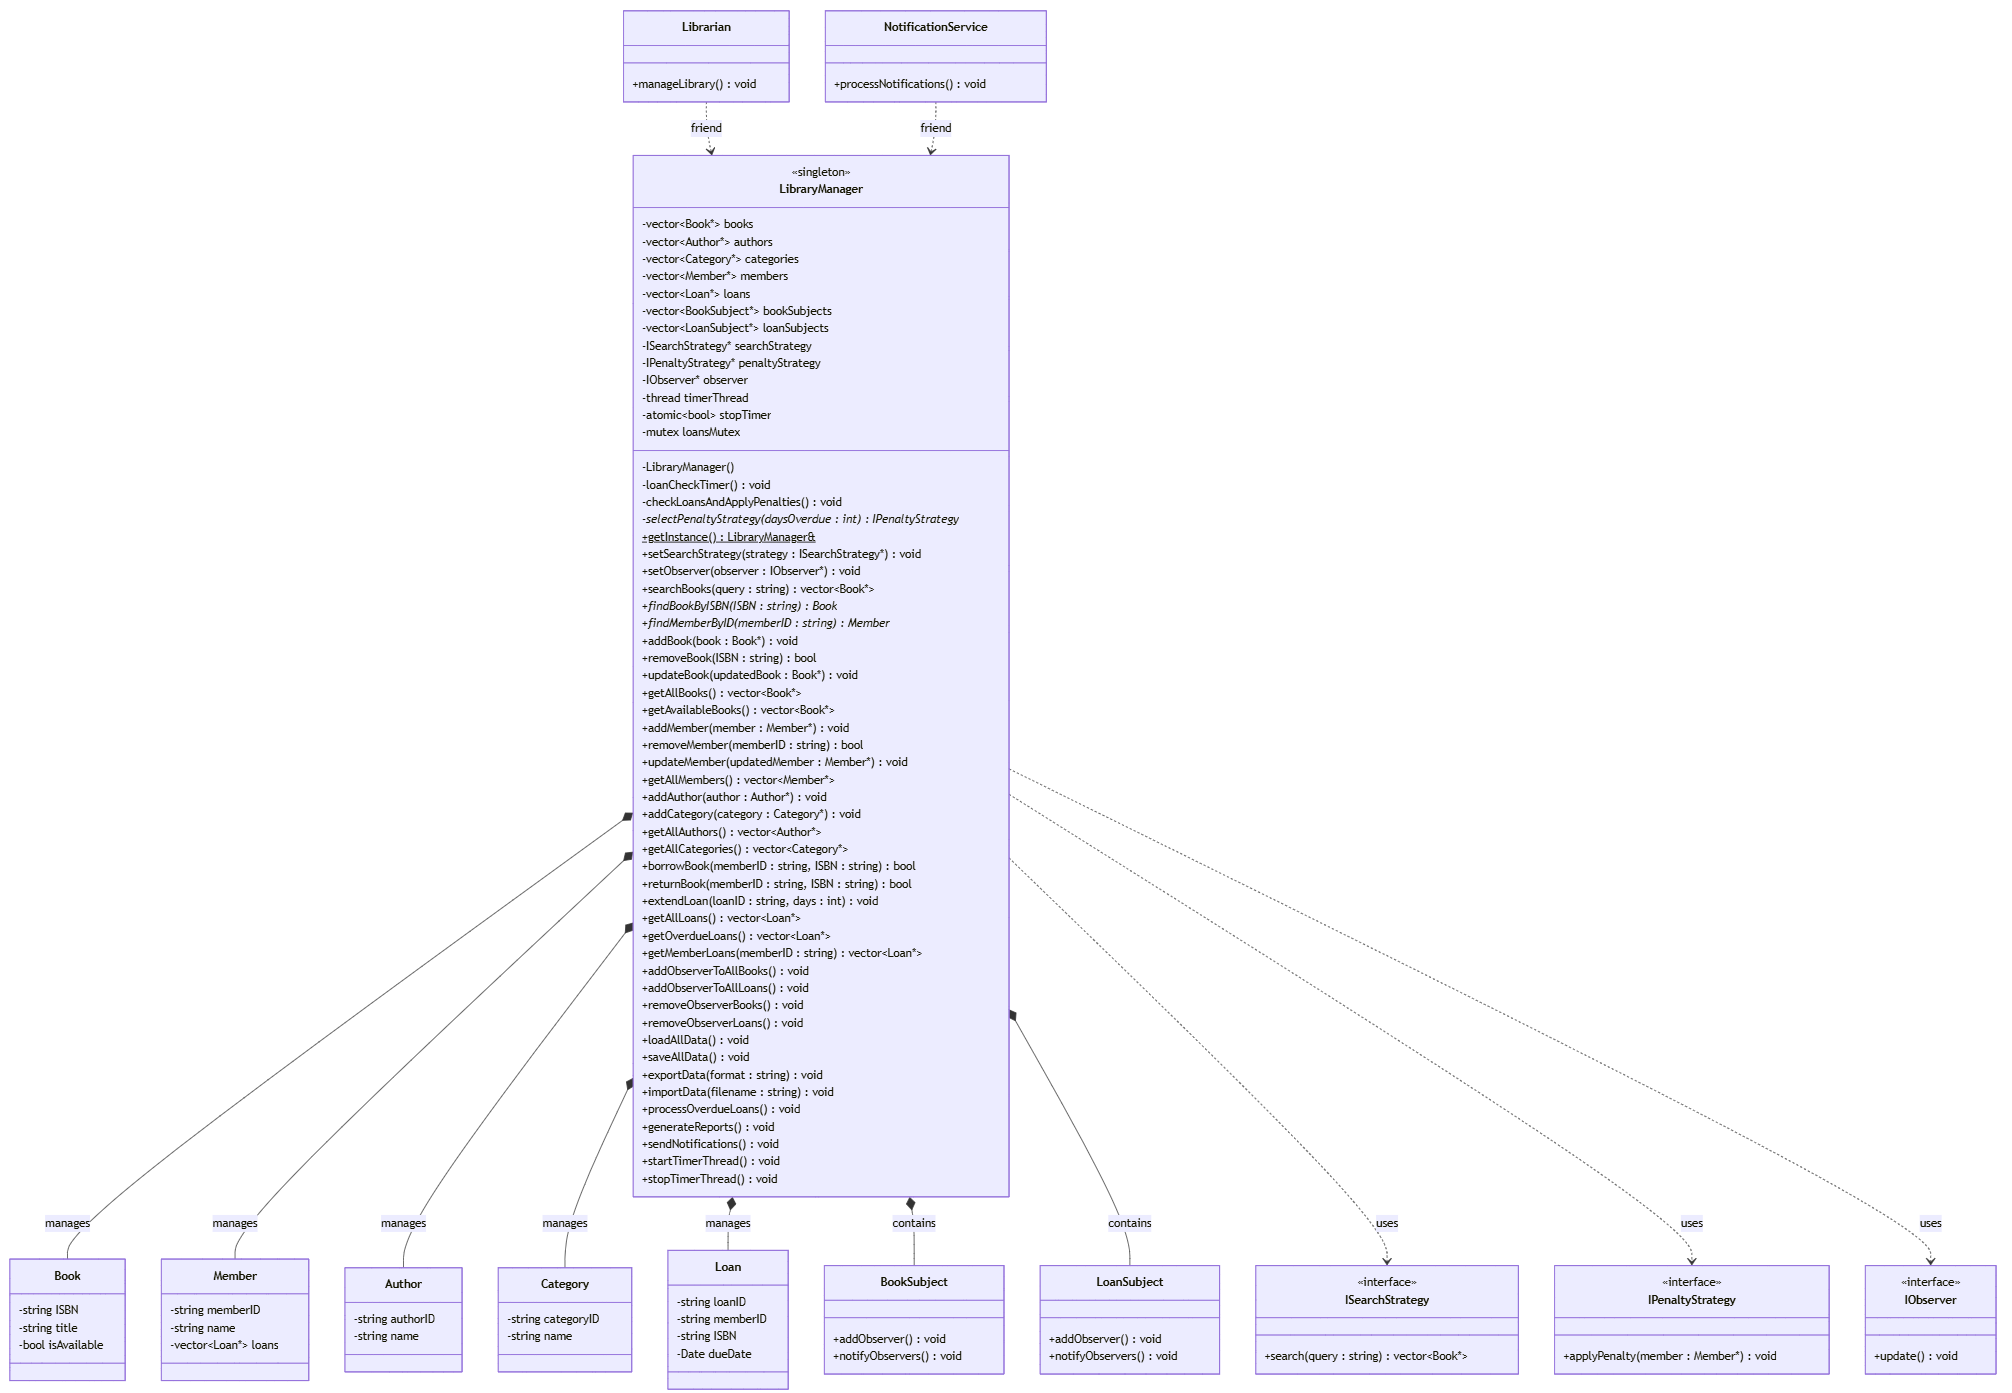
\includegraphics[width=0.7\textwidth]{figures/singleton_pattern.png}
    \caption{UML Diagram for the Singleton Pattern.}
    \label{fig:singleton_pattern}
\end{figure}

\subsection{Observer Pattern}
\subsubsection{Purpose}
The Observer pattern defines a one-to-many dependency between objects. When one object (the "subject") changes its state, all its dependents (the "observers") are notified and updated automatically. This pattern is ideal for creating distributed event-handling systems.

\subsubsection{Implementation}
The Observer pattern is the backbone of the \texttt{NotificationService}. In our system, entities like \texttt{Loan} act as subjects. Observers, such as a \texttt{MemberObserver} or \texttt{LibrarianObserver}, can register themselves with a subject. When a loan's status changes (e.g., becomes overdue), the loan subject notifies all its registered observers, allowing the system to send alerts or take other actions without tightly coupling the \texttt{Loan} class to the notification logic.

\begin{figure}[H]
    \centering
    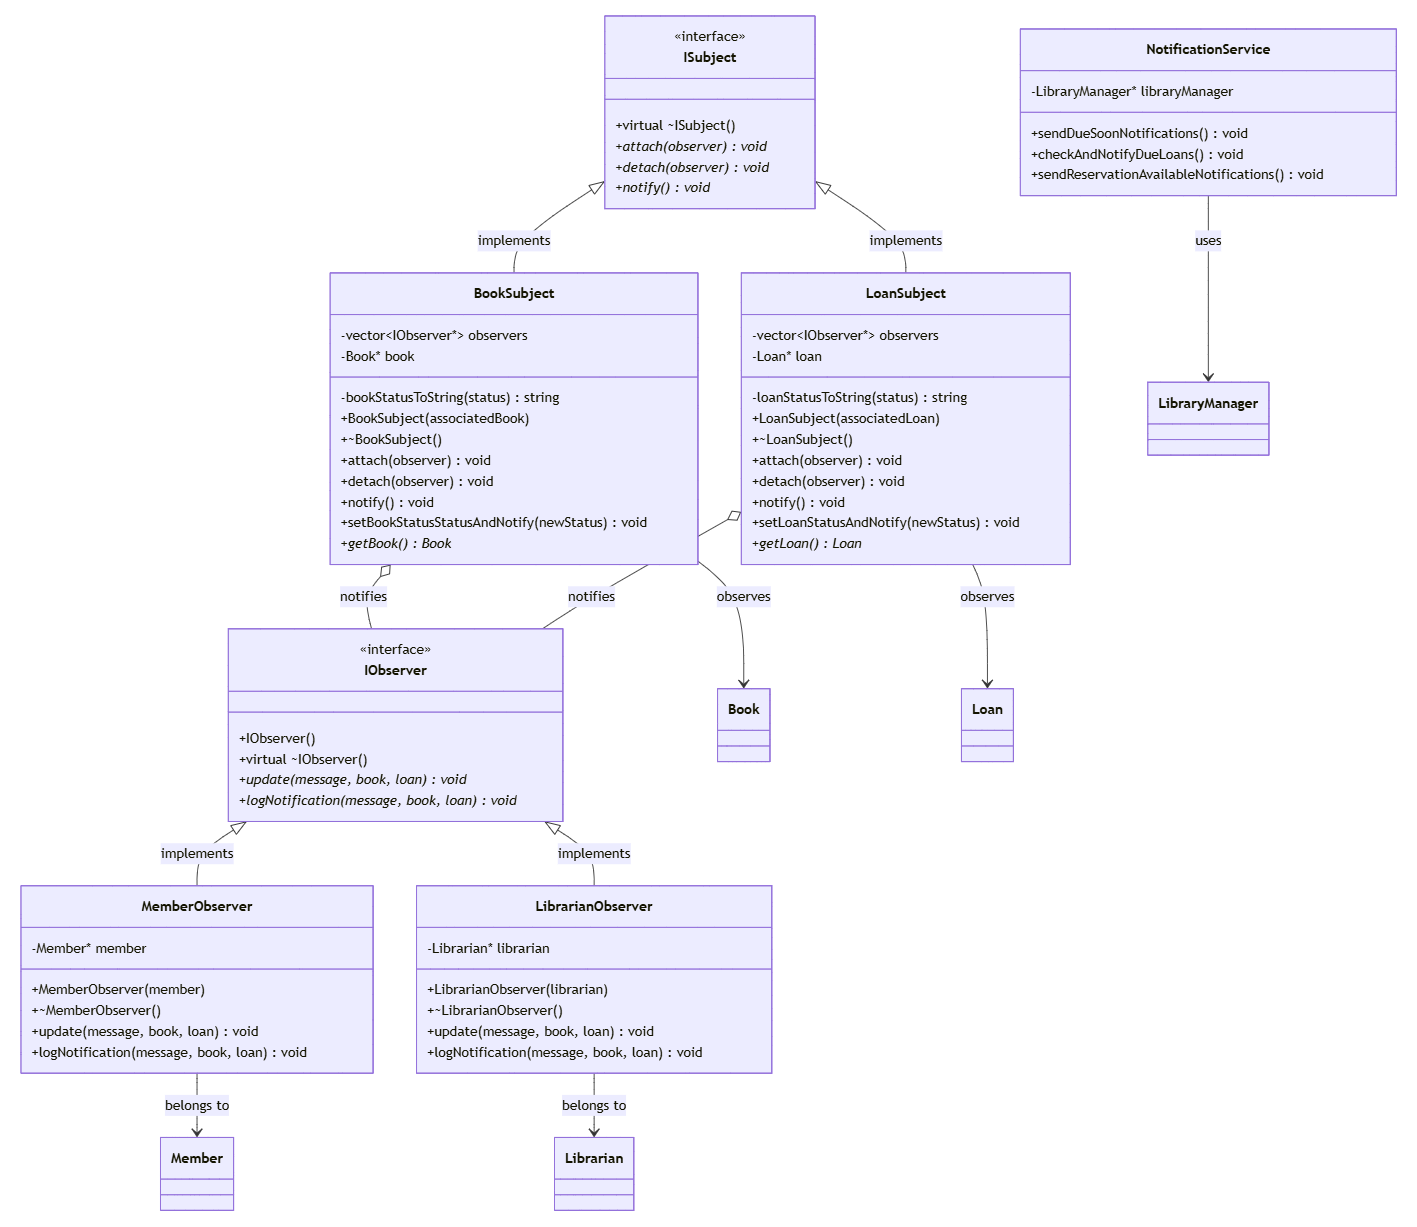
\includegraphics[width=\textwidth]{figures/observer_pattern.png}
    \caption{UML Diagram for the Observer Pattern.}
    \label{fig:observer_pattern}
\end{figure}

\subsection{Strategy Pattern}
\subsubsection{Purpose}
The Strategy pattern defines a family of algorithms, encapsulates each one, and makes them interchangeable. It lets the algorithm vary independently from the clients that use it. This is useful when you have multiple ways to perform a task and want to choose one at runtime.

\subsubsection{Implementation}
The Strategy pattern is used for implementing the book search functionality. An abstract interface, \texttt{ISearchStrategy}, defines a common \texttt{search()} method. Concrete strategy classes like \texttt{TitleSearchStrategy} and \texttt{AuthorSearchStrategy} implement this interface, each providing a different search algorithm. The client code can then select and use the desired search strategy at runtime without being coupled to its specific implementation.

% --- [HÌNH ẢNH] Sơ đồ cho Strategy Pattern ---
\begin{figure}[H]
    \centering
    % Hãy tạo một ảnh tên là 'strategy_pattern.png' và đặt nó vào thư mục 'figures'
    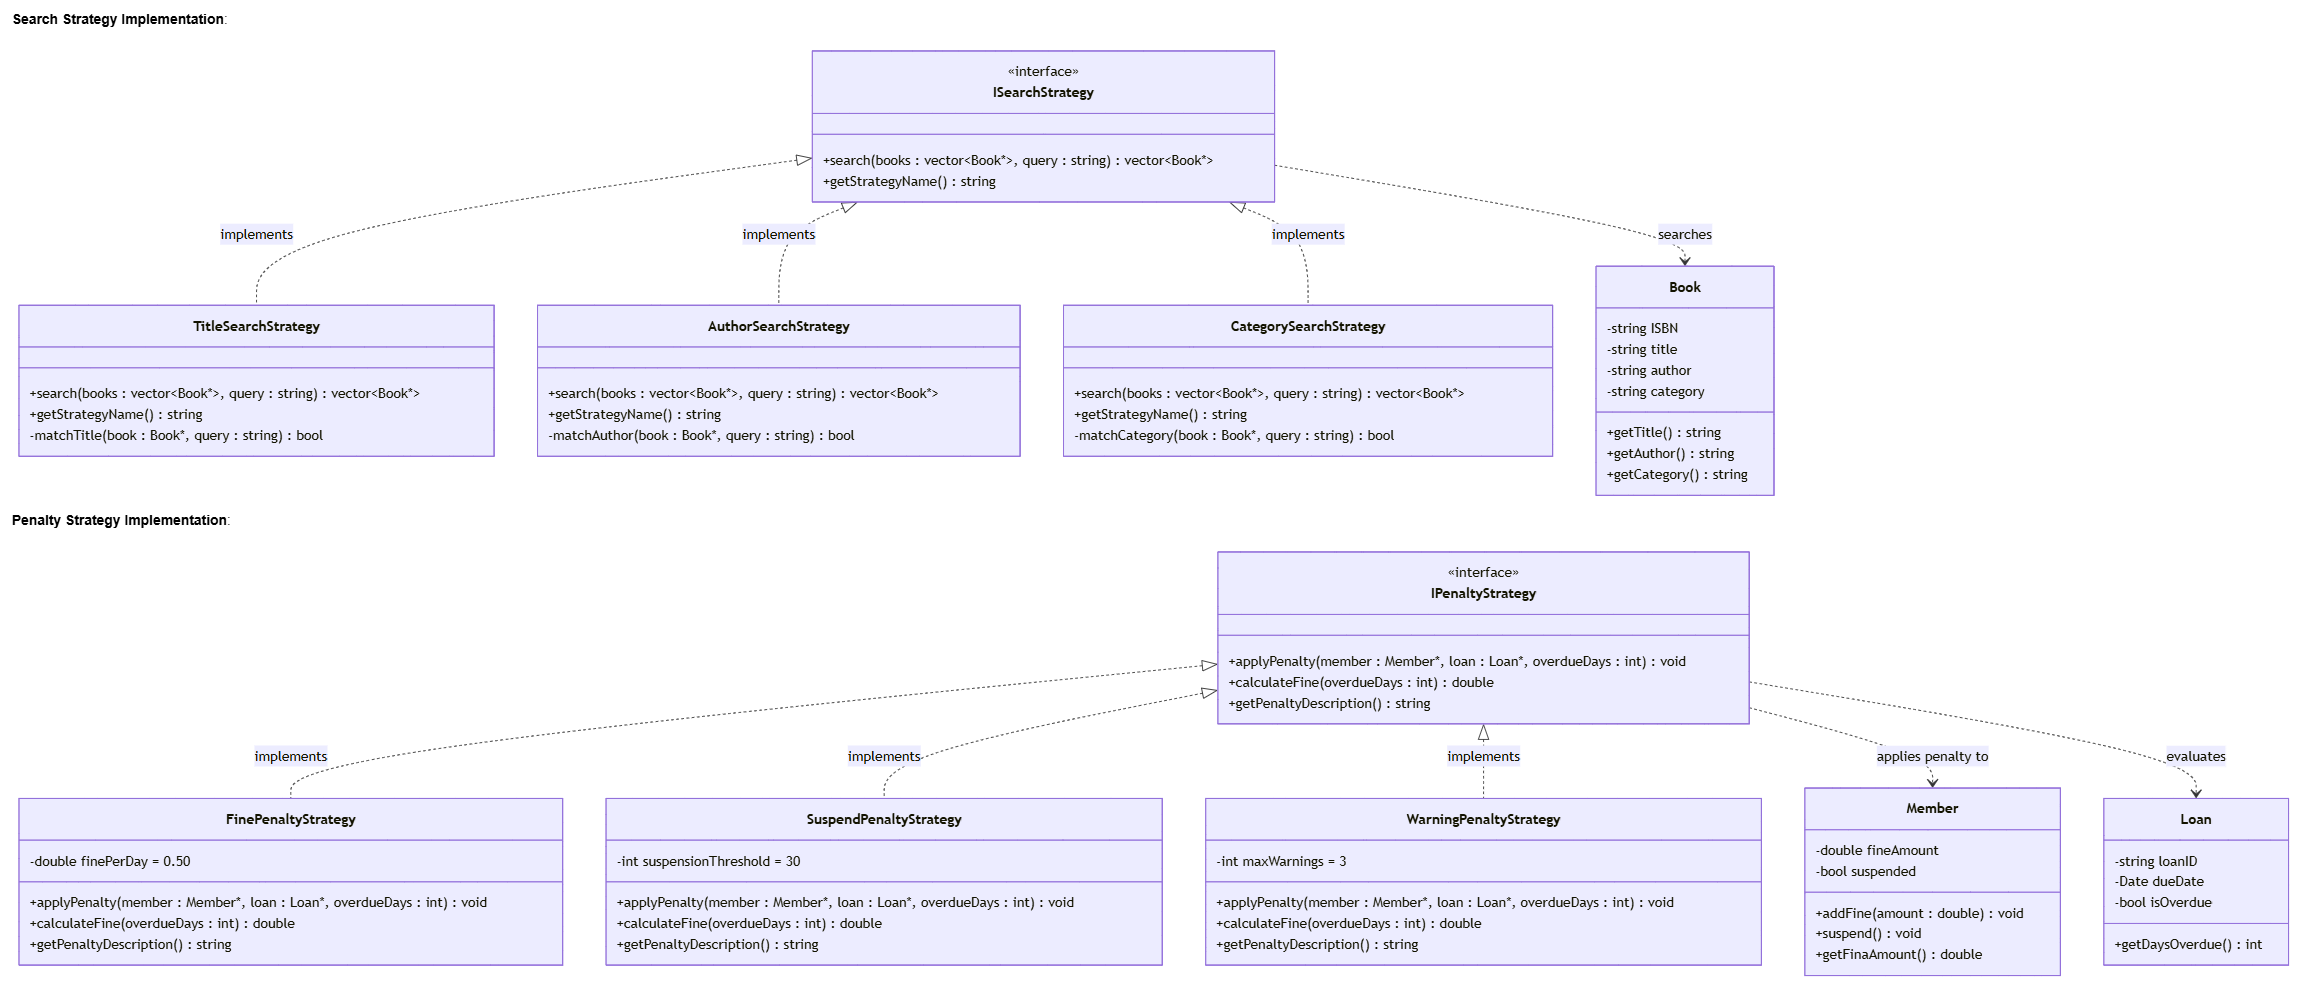
\includegraphics[width=\textwidth]{figures/strategy_pattern.png}
    \caption{UML Diagram for the Strategy Pattern.}
    \label{fig:strategy_pattern}
\end{figure}

\subsection{Decorator Pattern}
\subsubsection{Purpose}
The Decorator pattern allows behavior to be added to an individual object, either statically or dynamically, without affecting the behavior of other objects from the same class. It is used to extend an object's functionality.

\subsubsection{Implementation}
This pattern is used to add extra information to \texttt{Book} objects in a flexible way. A base \texttt{BookDecorator} class inherits from \texttt{Book} and also contains a pointer to a \texttt{Book} object. Concrete decorator classes like \texttt{DifficultyLabelDecorator} and \texttt{SpecialTagDecorator} inherit from \texttt{BookDecorator}. They override methods like \texttt{getFullDescription()} to first call the wrapped object's method and then add their own information (e.g., a difficulty label or a "Bestseller" tag) to the result.

\begin{figure}[H]
    \centering
    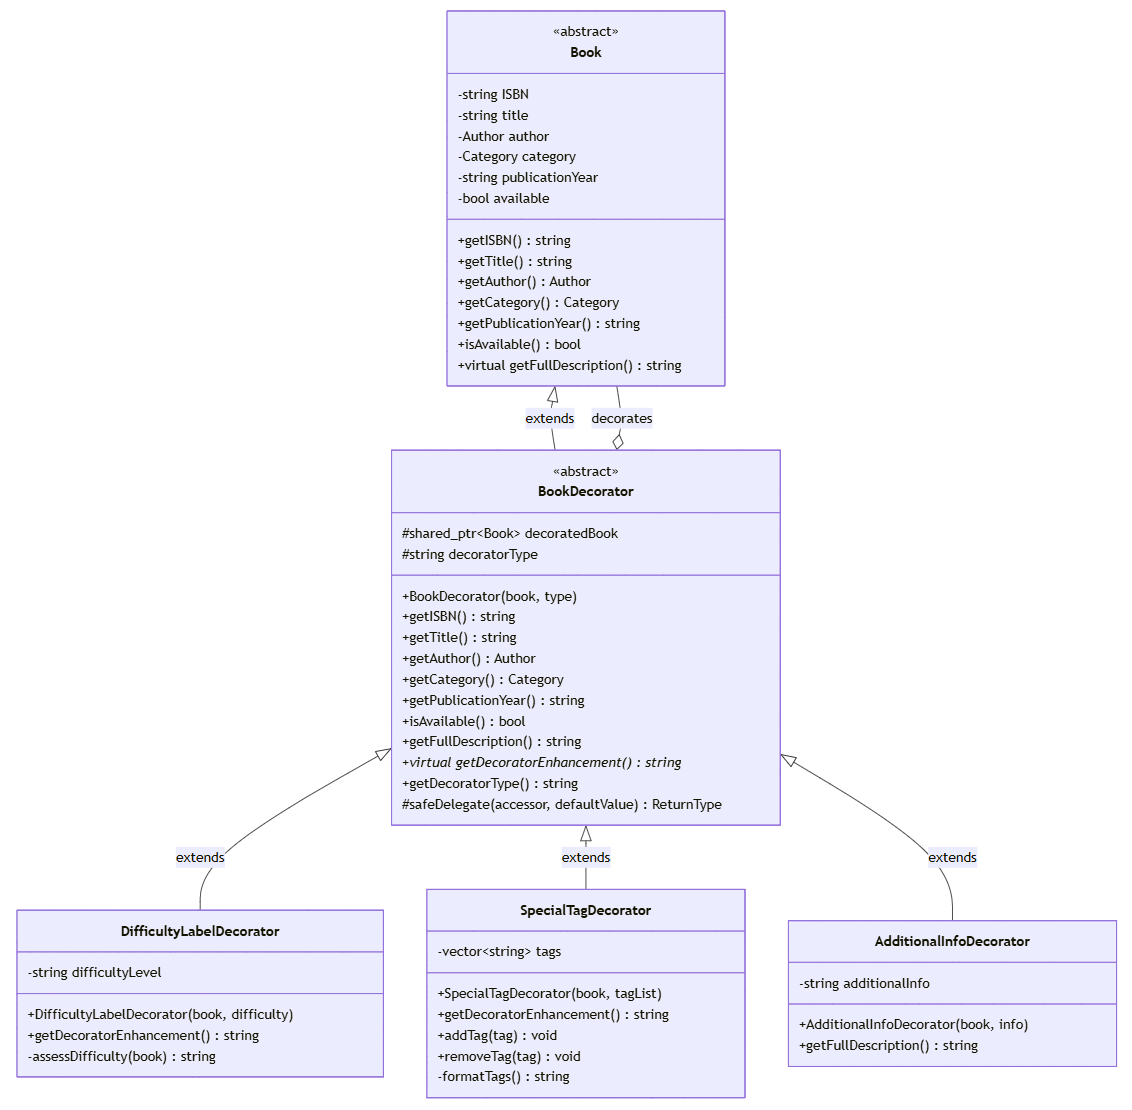
\includegraphics[width=\textwidth]{figures/decorator_pattern.png}
    \caption{UML Diagram for the Decorator Pattern.}
    \label{fig:decorator_pattern}
\end{figure}